
\section{Class Introduction}
\subsection{Outline}

\begin{frame}
  \centering
  {\huge
    What is the objective of this course
  }
\end{frame}

\begin{frame}
  \frametitle{Outline}
  \begin{enumerate}
    \item Course Objective
    \item What is a Programming Challenge?
    \item Course Topics
    \item Lecturer Introduction
    \item Extra: ICPC
  \end{enumerate}
\end{frame}

\subsection{Class Objective}
\begin{frame}{Class Objective}
  \begin{itemize}
    \item Course Objective: \alert{Improve your algorithm skill by writing many programs};
    \bigskip

    \item \alert{Key Idea:} Write programs that solve challenges (puzzles)
    \begin{enumerate}
      \item Read the problem and understand the puzzle;
      \item Choose the algorithm and implement;
      \item Run the program and check the correct result;
      \item Repeat many times
    \end{enumerate}
    \medskip

    \item In this lecture, we want to \alert{use in practice} the algorithms that we
    learned in the 1st and 2nd year.
  \end{itemize}
\end{frame}

\begin{frame}{Algorithms: Theory vs. Implementation}
  \begin{exampleblock}{}
  Why is this a good idea? When we apply a textbook algorithm to a puzzle, we learn many new things:
  \end{exampleblock}
  \begin{itemize}
    \item \alert{Input/Output}: How to transform the input data to a format that the algorithm understands;
    \item \alert{Input Size}: If the input is very large, a wrong program or algorithm can be very slow;
    \item \alert{Special Cases}: How to think about special cases that can cause bugs or errors in the program;
    \item \alert{Debugging}: How to find the source of bugs in your program, specially if the bug is because of a {\bf special case?};
  \end{itemize}
\end{frame}

\begin{frame}{Automated Judging}
  \begin{exampleblock}{}
  In this lecture we use {\bf Automated Judges (AJ)} to check if your homework is correct.
  \end{exampleblock}

  \begin{itemize}
    \item An AJ is a website that proposes programming puzzles, and receive solutions;
    \begin{itemize}
      \item Ex: AtCoder, Aizu Online Judge, Topcoder, Codeforces, etc.
    \end{itemize}\bigskip

    \item The AJ receives your program; compile it; and grade it;\bigskip

    \item The AJ test your program with a set of \structure{Hidden Inputs}\bigskip

    \item The AJ gives you the result: \structure{Correct} or \alert{Incorrect}
    \begin{itemize}
      \item If the result is incorrect, it will not tell you why;
      \item You have to create debug cases by yourself;
      \item But, you can submit a new version as many times as you want;
    \end{itemize}
  \end{itemize}
\end{frame}

\begin{frame}{What this class expects of you}
  \begin{exampleblock}{Estimated classwork:}
    \begin{itemize}
      \item You need basic programming knowledge (in C, C++, Java or Python);
      \medskip

      \item Complete 2 or more program assignments per week;
      \begin{itemize}
        \item Average of 4 hours of study per week;
        \item A lot of time with debug and creating test cases;
        \item (Atcoder difficulty: 300 to 500)
      \end{itemize}
      \medskip

      \item Homework starts easy, but becomes harder later in the course;
      \medskip

      \item No final exam: only assignments!
    \end{itemize}
  \end{exampleblock}
  \hfill {\bf Hint: Do your homework early!}
\end{frame}

\subsection{What are Programming Challenges?}
\begin{frame}{What kind of assignment?}
  A "Programming Challenge" is a puzzle problem that needs to be solved by writing
  a program.\vfill

  The program {\bf reads the input}, and must write the {\bf correct output},
  following the rule of the puzzle {\bf exactly}.\vfill

  {\bf You don't know all the input}. You must make sure that your program
  can solve {\bf Any acceptable input}.\vfill

  There is a {\bf running time limit} so your program must be efficient.\vfill

  In general, a correct program will be small (< 200 lines).
\end{frame}


\begin{frame}{Why programming challenges?}
  \begin{itemize}
    \item {\bf For Competitions}: Around 1980, Programming Contests started as a way for Computer Sciences universities to compete. (IOI, ICPC, etc)
    \bigskip

    \item {\bf For Study}: After 2000, many people use online Automated Judges to study programming and prove their ability; (TopCoder, Codeforces, AtCoder, etc);
    \bigskip

    \item {\bf For Recruitment}: Recently, many companies use Programming Challenges to test the programming ability of candidates. candidates. (Google, Facebook, etc)\bigskip

    \item {\bf For Fun}: Some people just like to have an excuse to program!
  \end{itemize}
\end{frame}

\subsection{Example}
\begin{frame}{Example: The 3n+1 problem}
  \begin{columns}
    \column{0.55\textwidth}
      Contents of a Programming Challenge:
      \begin{itemize}
        \item Problem Description;
        \item Input Description;
        \item Output Description;
        \item Input/Output Example;
      \end{itemize}

    \column{0.45\textwidth}
    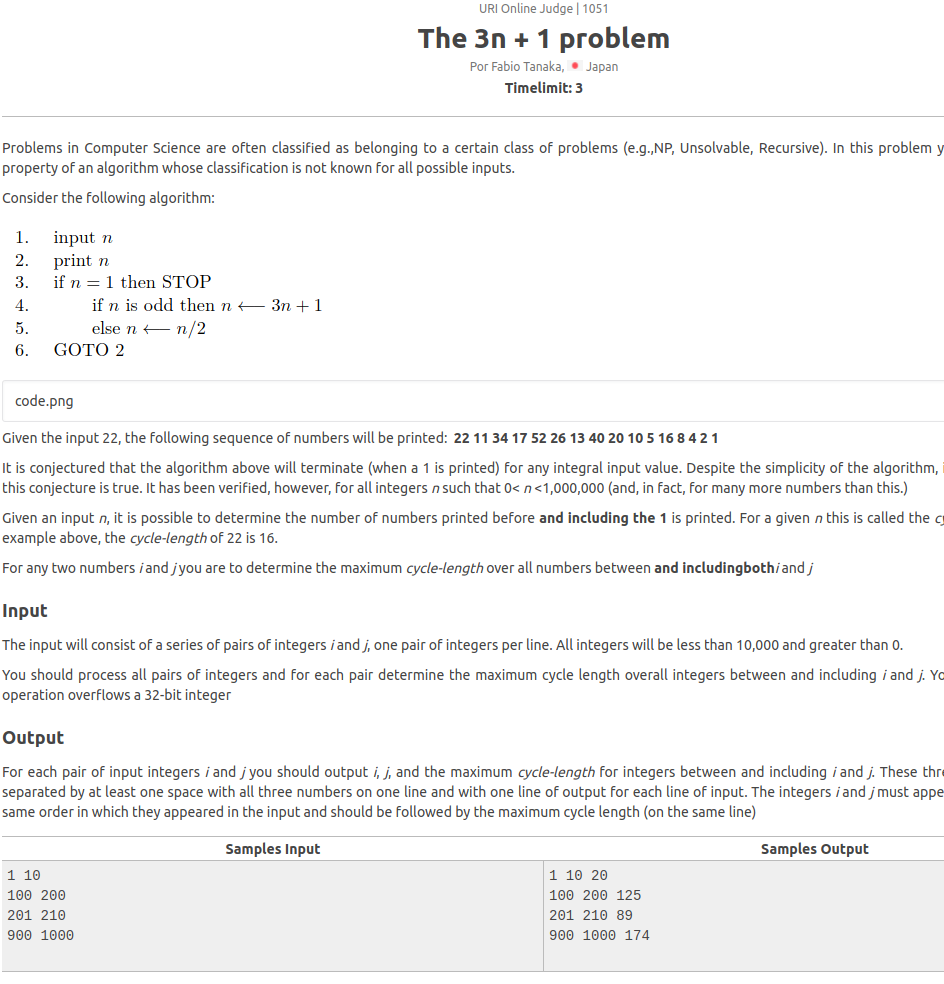
\includegraphics[width=1\textwidth]{img/3n_problem}
  \end{columns}
\end{frame}

\begin{frame}{Example: The 3n+1 problem}{What is the problem?}
  \begin{columns}
    \column{0.55\textwidth}
    {\smaller
    The problem wants the \structure{longest sequence size} generated by the following algorithm:
      \begin{enumerate}
        \item if $n = 1$ then STOP
        \item if $n$ is odd, then $n = 3n + 1$
        \item else $n = n/2$
        \item GOTO 1
      \end{enumerate}
    \medskip

    For example, if $i = 1$ and $j = 4$:
    \begin{itemize}
      \item n = 1: 1 END; {\bf Length 1}
      \item n = 2: 2 1 END; {\bf Length 2}
      \item n = 3: 3 10 5 16 8 4 2 1 END; {\bf Length 8}
      \item n = 4: 4 2 1 END; {\bf Length 3}
    \end{itemize}
    So the {\bf maximum length} is 8 (for n = 3)}
    \column{0.45\textwidth}
    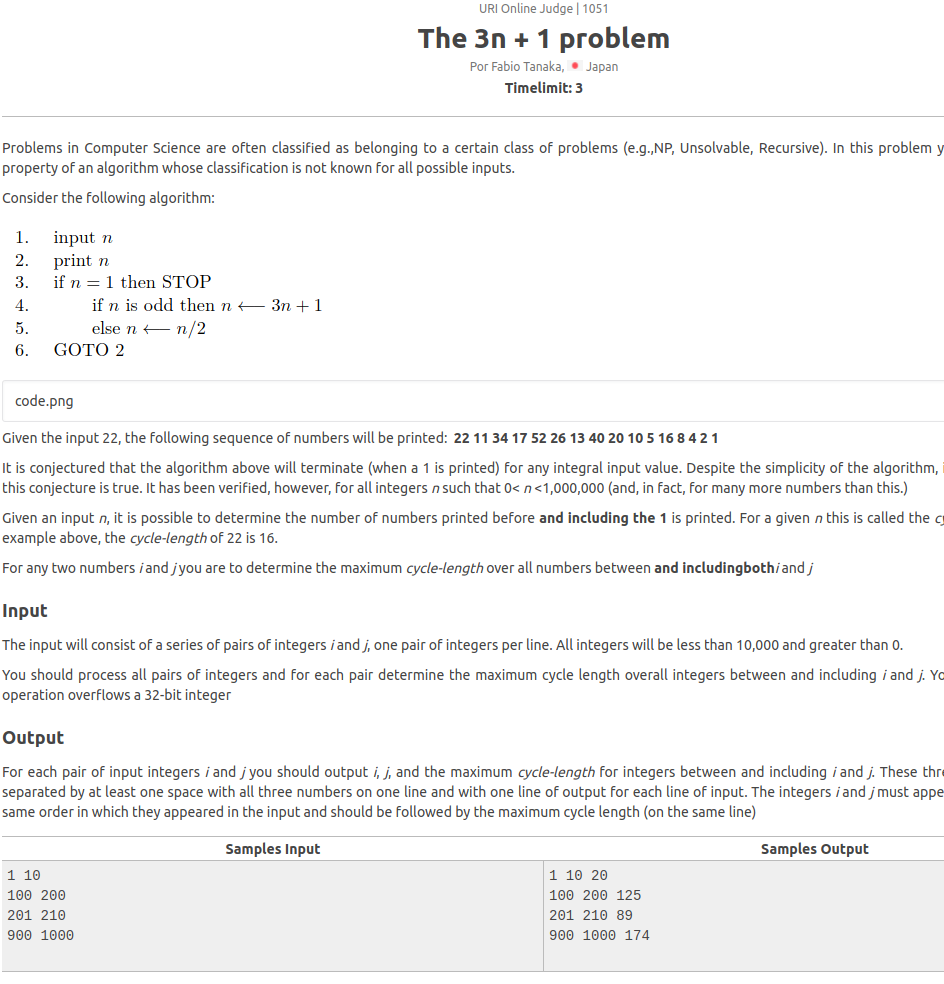
\includegraphics[width=1\textwidth]{img/3n_problem}
  \end{columns}
\end{frame}

\begin{frame}[fragile]{Example: The 3n+1 problem}{A simple program}
{\smaller
\begin{verbatim}
int main() {
  int min, max;
  int maxcycle = 0;
  cin >> min >> max;
  for (int i = min; i <= max; i++) {
    int cycle = 1;
    int n = i;
    while (n != 1) {
      if (n % 2 == 0) { n = n / 2; }
      else { n = n*3 + 1; }
      cycle++;
    }
    if (cycle > maxcycle) maxcycle = cycle;
  }
  cout << min << " " << max << " " << maxcycle << "\n";
  return 0;
}
\end{verbatim}}
\end{frame}

\begin{frame}{Example: The 3n+1 problem}{Simple programs, simple
  problems}

If you try to run this program with large inputs, it will be very slow! Why?
\bigskip

i = 1, j = 10:
\begin{itemize}
  \item n = 1: 1 END
  \item n = 2: 2 1 END
  ...
  \item n = 7: 7 22 11 34 17 52 26 13 40 20 10 5 16 8 4 2 1 END\\
  ...
  \item n = 9: 9 28 14 \alert{7 22 11 34 17 52 26 13 40 20 10 5 16 8 4 2 1 END}
  \item n = 10: \alert{10 5 16 8 4 2 1 END}
\end{itemize}
\bigskip

A lot of work is repeated without necessity. How to make the program faster?
\end{frame}

\begin{frame}{Example: The 3n+1 problem}{Memoization}
  A technique called {\bf Memoization} can solve the "repeated work" problem.
  \bigskip

  {\bf Memoization}:
  \begin{itemize}
    \item Every time you finish a calculation, store the result in the memory;
    \item Before you begin a calculation, check if it is not in the memory;
  \end{itemize}
  \bigskip

  This technique can reduce the amount of repeated work.
  \bigskip

  In this course we will review and study many techniques like this one. You will have to implement these techniques in the homework to make it efficient.
\end{frame}

\subsection{Class Program}
\begin{frame}{Topics in this course}
  \begin{enumerate}
    \item Introduction
    \item Data Structures
    \item Search Problems
    \item Dynamic Programming
    \item Graphs Problems (Graph Structure)
    \item Graph Problems (Graph Search and Flow)
    \item String Manipulation
    \item Math Problems
    \item Geometry Problems
    \item Final Remix
  \end{enumerate}
\end{frame}

\subsection{Lecturer Introduction}
\begin{frame}
  \frametitle{About the Lecturer}
  \begin{columns}
    \column{0.4\textwidth}
    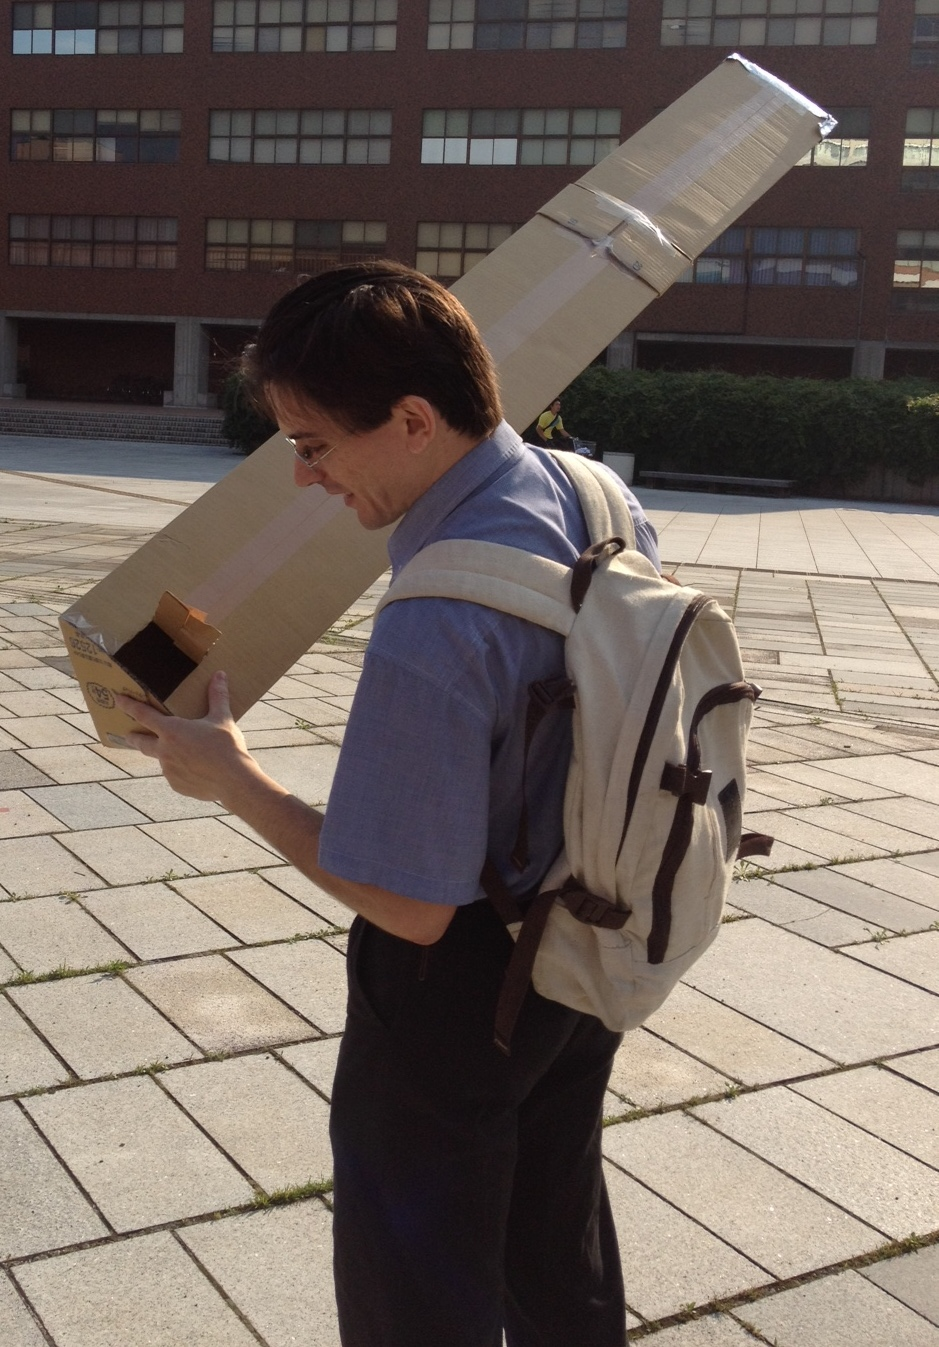
\includegraphics[height=.8\textheight]{../img/pinhole}
    \column{0.6\textwidth}
    {\small
    \begin{itemize}
      \item \structure{Name:} Claus Aranha;
      \item \structure{Country:} Brazil;
      \item \structure{Research Topics:}
      \begin{itemize}
        \item Evolutionary Computation;
        \item Artificial Life;
      \end{itemize}
      \item \structure{Hobbies:}
      \begin{itemize}
        \item Game Programming;
        \item Geocaching;
      \end{itemize}
        \medskip

      \item \structure{webpage:}\\ {\smaller \url{http://conclave.cs.tsukuba.ac.jp}}
    \end{itemize}
    }
  \end{columns}
\end{frame}

\subsection{ICPC}
\begin{frame}{Extra: Join the Tsukuba ICPC Team!}{What is ICPC?}
  \hfill 
\includegraphics[width=0.4\textwidth]{img/icpclogo}\\
  If you like these contests, and want an extra challenge, please consider
  joining the Tsukuba ICPC team!
  \bigskip

  ICPC (International Collegiate Programming Contest) is the largest and
  most traditional programming competition between universities.
  \bigskip

  More than 50.000 students from all over the world participate in this
  competition every year.
  \bigskip

  Contest Website: \url{https://icpc.baylor.edu/}
\end{frame}

\begin{frame}{Extra: Join the Tsukuba ICPC Team!}{Program and see the world!}
  \hfill 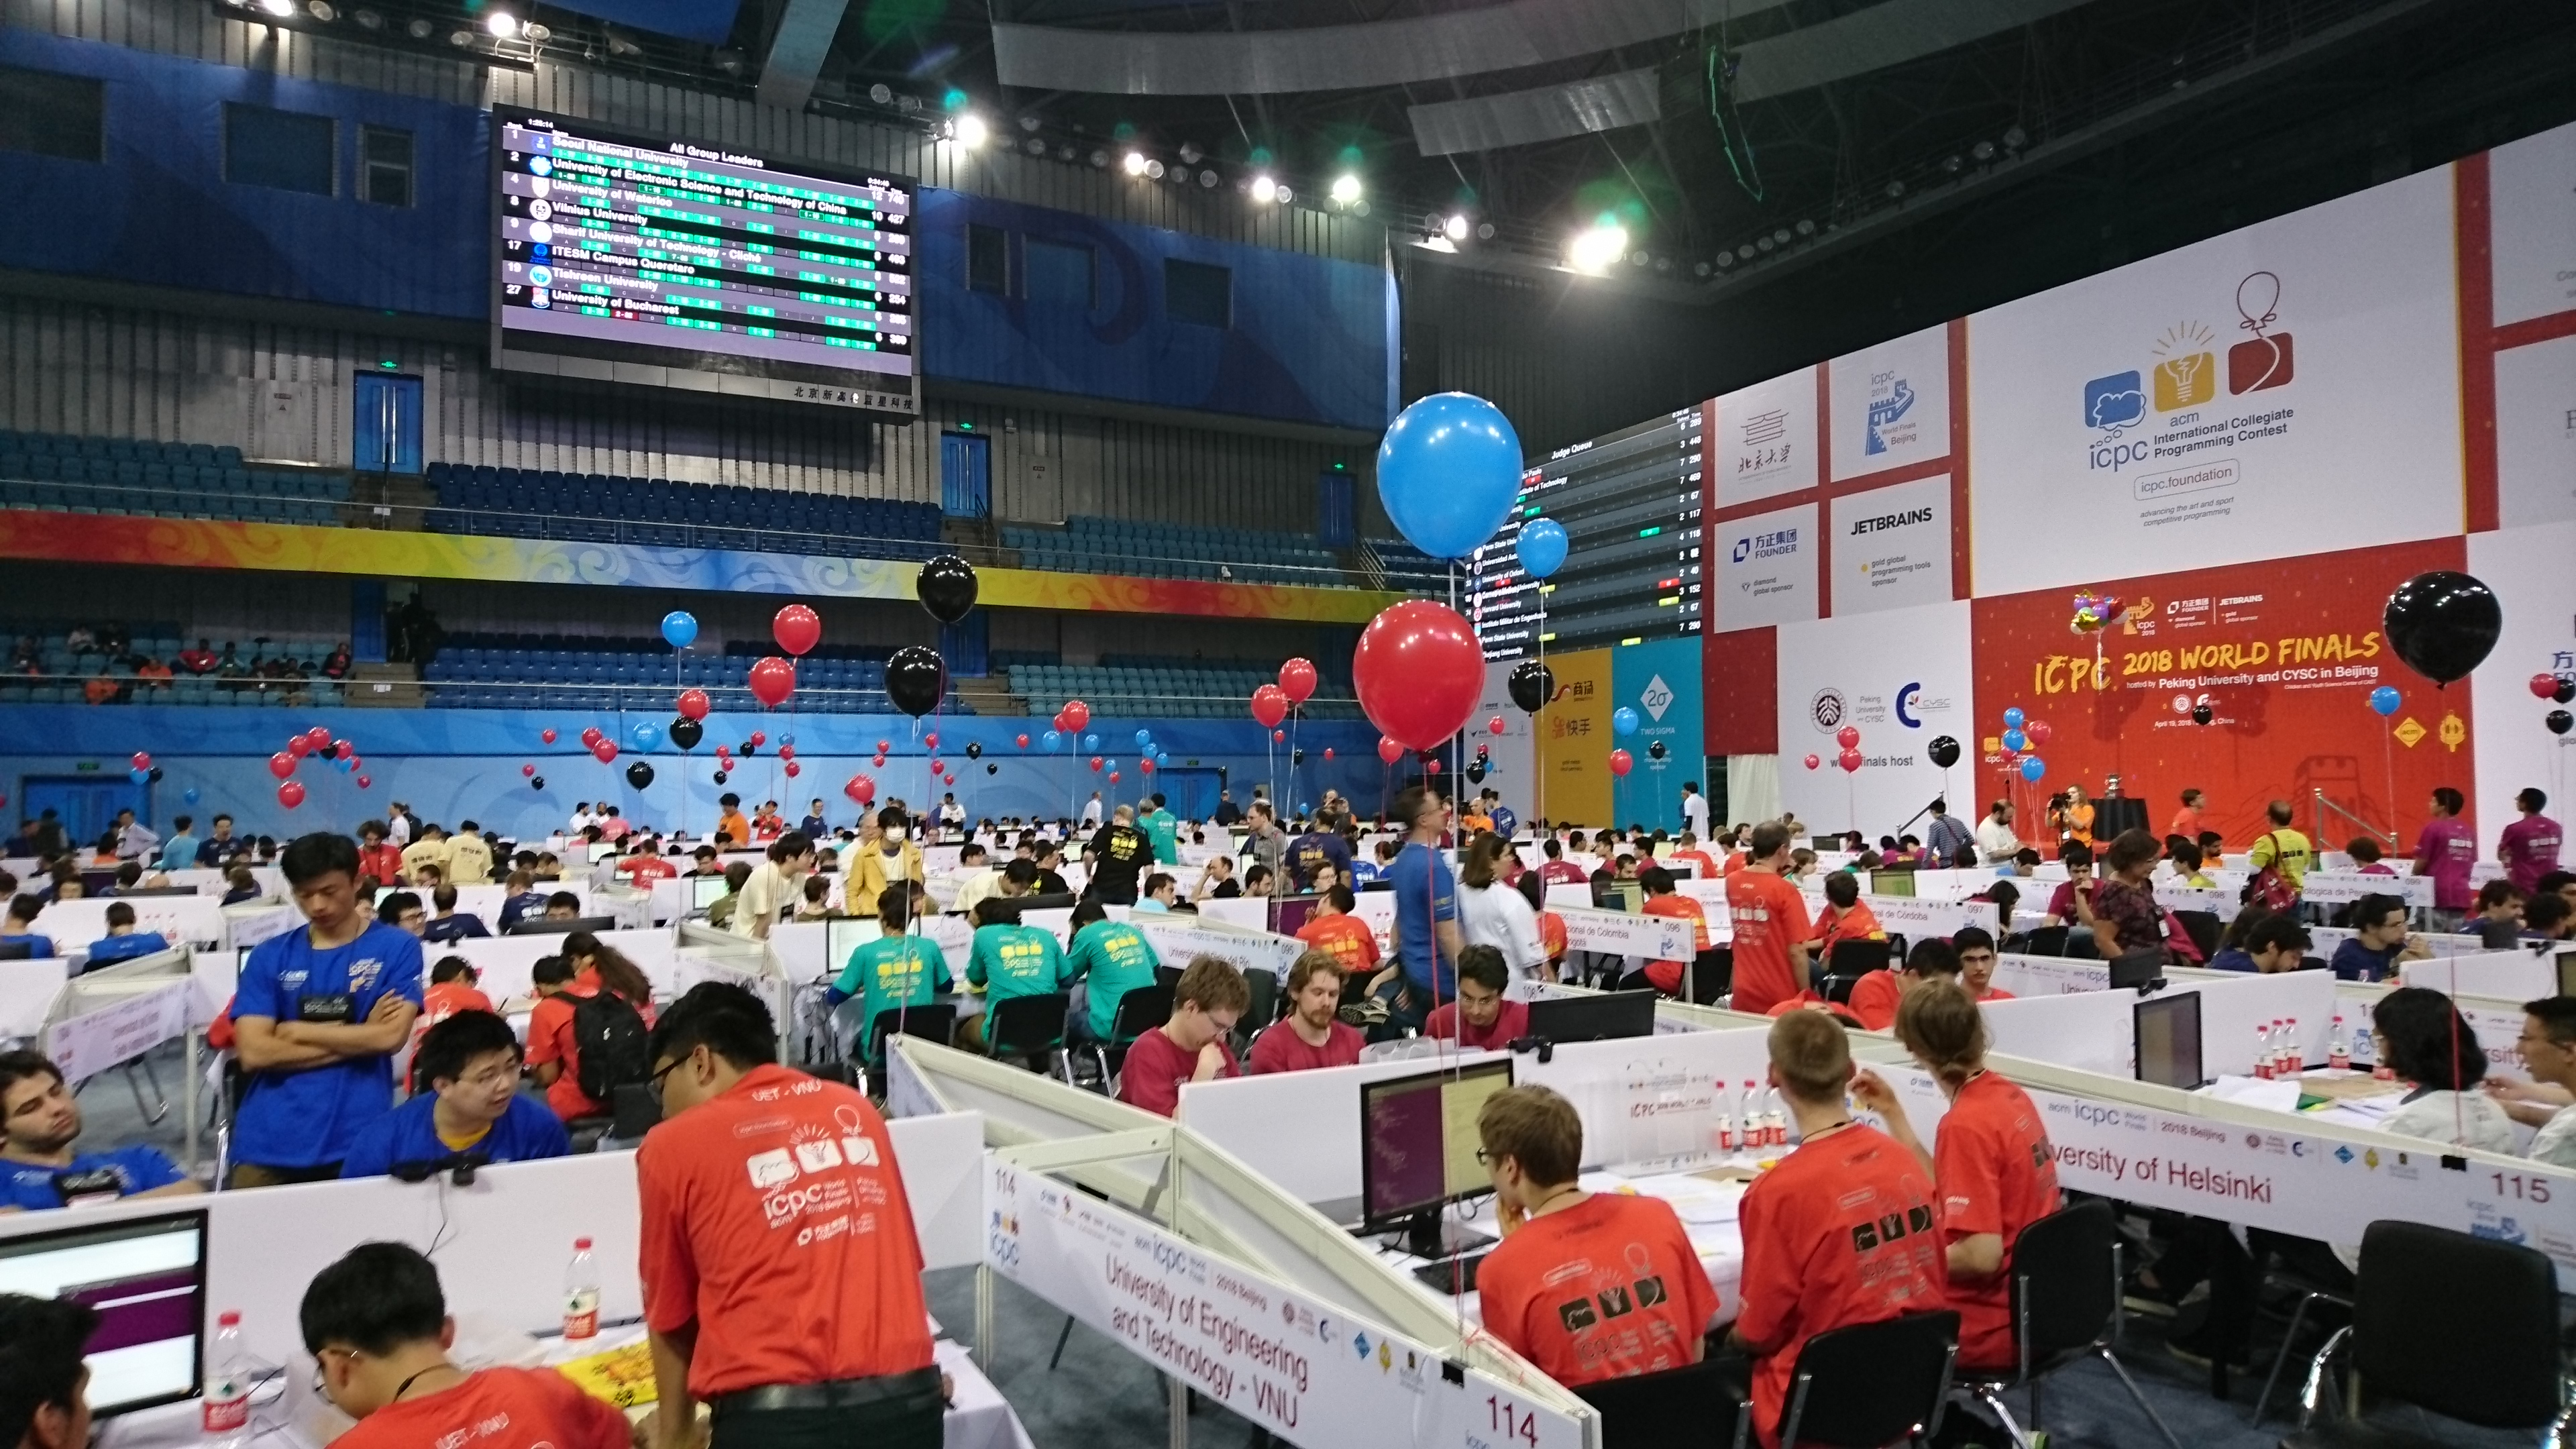
\includegraphics[width=0.4\textwidth]{img/icpc_image1}
  \begin{itemize}
    \item \alert{Requirements}: Team of 3 students, any course;
    \medskip

    \item \alert{Schedule:}
    \begin{itemize}
      \item National Preliminary Competition in July
      \item Japanese Regional Competition in October
      \item Asian Semi-final in December
      \item World Final April next year
    \end{itemize}
      (\alert{Dates may change this year because of nCov-19})
    \medskip
    \item Contact me if you're interested!
  \end{itemize}
\end{frame}



%%%%%%%%%%%%%%%%%%%%%%%%%%%%%%%%%%%%%%%%%%%%%%%%%%%%%%%%%%%%%%%%%%%%%%%%%%%%
